\chapter{Parameters identification}
\label{chap:paramidentification}
\section{Steady state analysis}
\label{sec:steadystate}
Using the data of the file \emph{data\_steps.mat}, we analysed the step response
of the system by going to check the relationships between the stiffness of the 
springs. 
And estimating a new coefficient for the voltage-to-force.
The estimate of a new voltage-to-force coefficient is carried out using the 
equation \eqref{eq:matrixform}:
\begin{equation} \label{eq:voltage-force}
	[K] x = \begin{bmatrix}
 			g_{\text{v}}	\\
 			0 	\\
 			0
 		\end{bmatrix} \cdot v
\end{equation}
and therefore from \eqref{eq:voltage-force} it is possible to derive:
\begin{equation} \label{eq:voltageforce}
	g_{\text{v}} = [K]^{-1} \cdot b
\end{equation}
Using the steady state value of the three output and the equation 
\eqref{eq:voltageforce} it is possible to evaluate the ratio of the stiffness 
of the springs with respect to  the nominal value of the third spring indicated 
with $k_3$, so it is possible to rewrite:
\begin{equation}
	\label{eq:gvestimate}
	k_3 \begin{bmatrix}
		x_1\\
		x_2\\
		x_3\\
	\end{bmatrix} = v \cdot
	\begin{bmatrix}
		g_{\text{v}} + g_{\text{v}} \cdot \frac{k_3}{k_1} + g_{\text{v}} \cdot 
		\frac{k_{3}}{k_{2}}\\
    		g_{\text{v}} + g_{\text{v}} \cdot \frac{k_{3}}{k_{2}}\\
    		g_{\text{v}}
    \end{bmatrix}
\end{equation}
From the above equation \eqref{eq:gvestimate} we obtain the results: nominal 
and estimated ratios between the stiffness of the springs as well as the 
coefficient voltage-to-force. 
The table \ref{tab:error} shows values and it is possible to appreciate in the 
last column the error made on the estimate of these values, according to the 
formulation:
\begin{equation}
	\label{eq:ratioerror}
	\text{\textbf{err}} = 100\cdot\frac{\text{computed}}{\text{nominal}}
\end{equation}
%
%
\begin{table}[ht]
\centering
	\begin{tabular}{lrrr}
	\toprule
						& nominal & computed & error [\%] \\
 	\midrule
 		ratio $k_{3}/k_{1}$	& 0.50000 & 0.48935 &	2.17651 \\
		ratio $k_{3}/k_{2}$	& 0.50000 & 0.52086 & 	4.00560 \\
		gain ratio $g_{\text{v}}$ & 5.25000 & 6.04866 &  15.21248	\\
	\bottomrule
	\end{tabular}
	\caption{Stiffnesses ratios and voltage-to-force coefficients}
	\label{tab:error}
\end{table}
%
\section{System identification}
\label{sec:sysidentification}
It is necessary to estimate the parameters of three \textsc{dof} system at simple 
identification, so that the impulse response is used to suppose that a model is 
based on a set of parameters, identifying the inputs as the initial force and 
conditions and the output of the system.
thus comparing the system response measured with that predicted by the model.
Defined a model for the system: depends on a set of parameters $\theta$. 
Identify the input (strength and i.c.) and output $(x(t))$ of the system. 
By giving the same input to the model and comparing the measured response $x(t)$ 
to that expected by the model $(x(t,\theta))$.
%
\begin{figure}[htb]
	\centering
	\resizebox{.50\linewidth}{!}{\begin{tikzpicture}
% help guide lines
%\draw[help lines] (0,0) grid [step = 5 mm](10,10);
%\foreach \x in {0,1,...,10}
%   \draw [help lines] (\x,0) node [below,%
%          font=\footnotesize] {$\x$} -- (\x,0);
%\foreach \y in {0,1,...,10}
%   \draw [help lines] (0,\y) node [left,%
%          font=\footnotesize] {$\y$} -- (0,\y);
%
% define model box
\newcommand{\modelbox}[2]{
	% input arrow  
	\coordinate (startarrow) at ({#1},{#2});
	\coordinate	(endarrow) at ($(startarrow)+(2.5,0)$);
	\draw [-stealth]($(startarrow) + (0,1 * 1)$) -- ($(endarrow)+(0,1* 1)$) node[above, midway] {$f(t)$};
	\draw [-stealth]($(startarrow) + (0,1 * 0)$) -- ($(endarrow)+(0,1* 0)$) node[above, midway, xshift=-0.65mm] {$\vec{x}_{0} \,, \dot{\vec{x}}_{0}$};
	% box
	% left low corner
	\coordinate (llcorner) at (2.5,-0.5);
	% right up corner
	\coordinate (rupcorner) at(6.5,1.5);
	\draw (llcorner) rectangle (rupcorner) node [midway]{dynamic system};
	% output arrow
	\coordinate (outputstartarrow) at (6.5,0.5);
	\coordinate	(outputendarrow) at (8.5,0.5);
	\draw [-stealth](outputstartarrow) -- (outputendarrow) node[above, midway] {$\vec{x}(t)$};
};
% 1 - plot the system model
\begin{scope}[yshift = 60mm]
   \modelbox{0}{0};  
\end{scope}
% 2 - plot second model and connection
\begin{scope}[yshift = 25mm]
   \modelbox{0}{0};
   \fill (1.75,1) circle (1.4pt);
   \fill (1,0) circle (1.4pt);
\end{scope}
% connect system model
   \draw (1.75,1) -- (1.75,3.5);
   \draw (1,2.5) -- (1,0);
% box model
\begin{scope}[xshift = 0mm]
   % input arrow  
	\coordinate (startarrow) at (1.75,1);
	\coordinate	(endarrow) at (2.5,1);
	\draw [-stealth](startarrow) -- (endarrow) node[below, midway] {$f(t)$};
	\draw [-stealth](1,0) -- (2.5,0) node[below, midway] {$\vec{x}_{0} \,, \dot{\vec{x}}_{0}$};
	% box
	% left low corner
	\coordinate (llcorner) at (2.5,-0.5);
	% right up corner
	\coordinate (rupcorner) at(6.5,1.5);
	\draw (llcorner) rectangle (rupcorner) node [midway]{model $\theta$};
	% output arrow
	\coordinate (outputstartarrow) at (6.5,0.5);
	\coordinate	(outputendarrow) at (8.5,0.5);
	\draw [-stealth](outputstartarrow) -- (outputendarrow) node[above, midway] {$\vec{x}(t)$};
\end{scope}
\end{tikzpicture}}
	\label{fig:systemmodel}
	\caption{System identification: real system and model}
\end{figure}
%
\\We define the residue as the difference between the two signals as in the 
equation \eqref{eq:residual}.
\begin{equation}
\label{eq:residual}
	\varepsilon(t,\theta) = x(t) - x(t,\theta)
\end{equation} 
The best choice for the set of parameter $\theta$ is the one that minimizes the 
residue integer (\ref{eq:residualinteger}) of the residue. 
\begin{equation}
\label{eq:residualinteger}
	\theta_{optim} = \text{argmin} \biggl( \int \varepsilon(t,\theta)^2 \, dt \biggr)
\end{equation} 
In this case, as the discrete signals with $N$ samples, the optimal value $N$ 
calculated as (\ref{eq:residualdiscrete}), this correspond to solving a least 
square problem.
\begin{equation}
\label{eq:residualdiscrete} 
\theta_{optim} = \text{argmin} \Biggl( \sum_{n=1}^{N} \varepsilon(t,\theta)^2 \Biggr)
\end{equation}

A linear model is adopted as described above, refer \ref{subsec:assumption}, 
assuming the stiffness matrix $[K]$ given.
Then quantifying the $[M]$ and $[C]$ parameters are used to minimize the problem.
Using the \emph{fmincon} algorithm, the problem is resolved. In addition, the 
selected algorithm is required to specify the lower and upper search limits; 
as well as the first guess conditons from which the result is strictly dependent.

\subsection{Free damping case}
\label{subsec:freedamping}
Using the data of the file \emph{data\_impulse.mat} identify the seven parameters
previously identified in the model and described by the equation \eqref{eq:matrixform}. 
In this case, since the response to impulse force, two to approximation of the 
force estimation, will be analysed, the voltage-to-force coefficient will be 
studied again.
The results of this optimization are shown in table \ref{tab:freedamping}.
\begin{table}[ht]
	\centering
	\begin{tabular}{SSSSSSS}
	\toprule
		\multicolumn{1}{c}%
			{$m_1$} & {$m_2$} & {$m_3$} & {$c_1$} &	 {$c_2$} & {$c_3$} & {$g_v$} \\
		\multicolumn{3}{c}{[\si{\kilo\gram}]}	&%
		\multicolumn{3}{c}{[\si{\newton\second\per\meter}]}	&%
		\multicolumn{1}{c}{[\si{\volt}]}\\
	\midrule
          1.5712  & 1.5020  & 1.2018  &  2.7956 &  1.9978 & 2.1950  &  1.2096	\\
    \bottomrule
	\end{tabular}
	\caption{Optimizations results in free damping case}
	\label{tab:freedamping}
\end{table}
\begin{figure}[htb]
	\centering
	\subfloat[][\emph{residual.}]
		{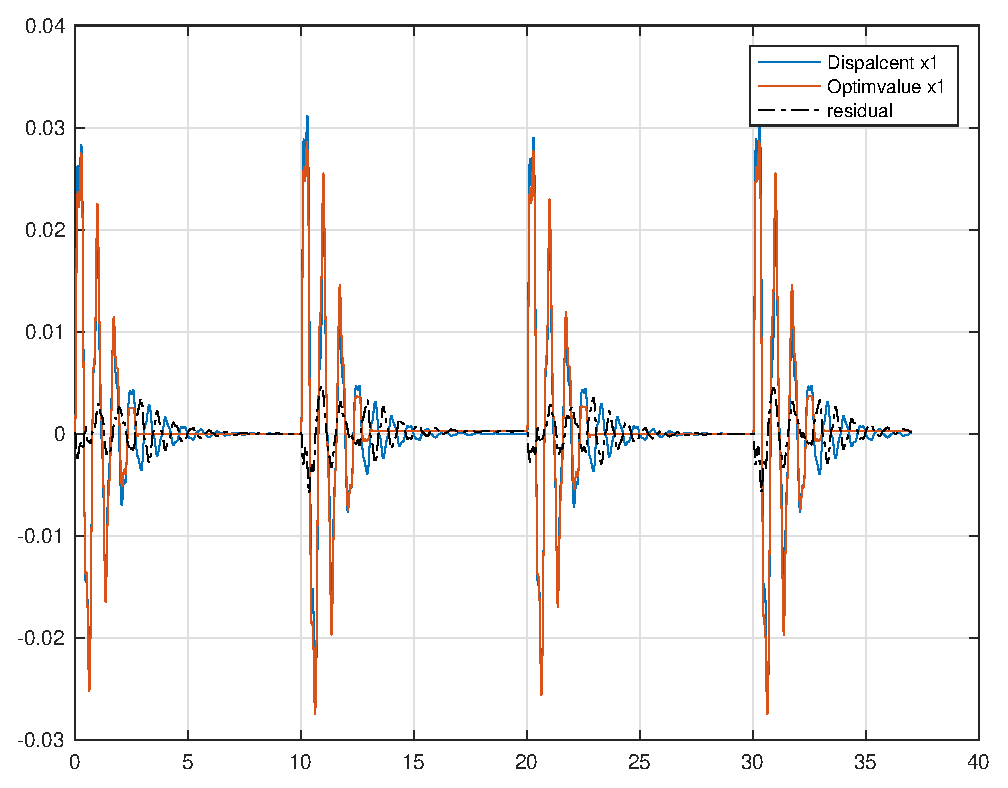
\includegraphics[width=0.45\textwidth]{residualfull1}}	\,
	\subfloat[][\emph{residual.}]
		{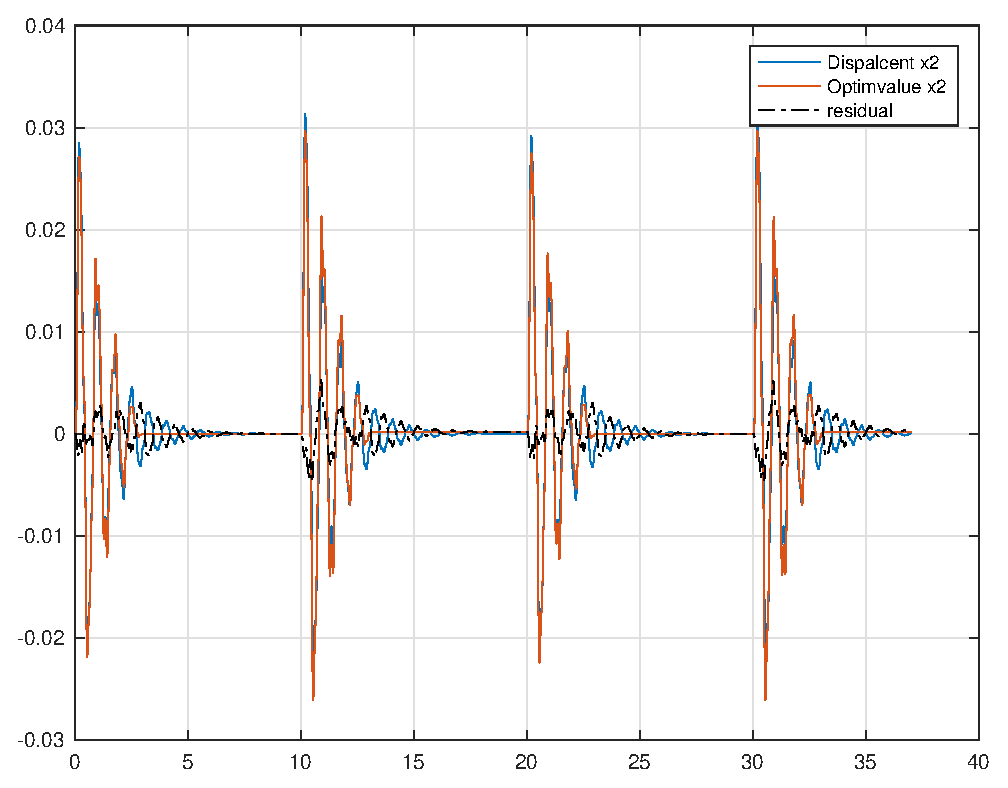
\includegraphics[width=0.45\textwidth]{residualfull2}}	\\
	\subfloat[][\emph{residual.}]
		{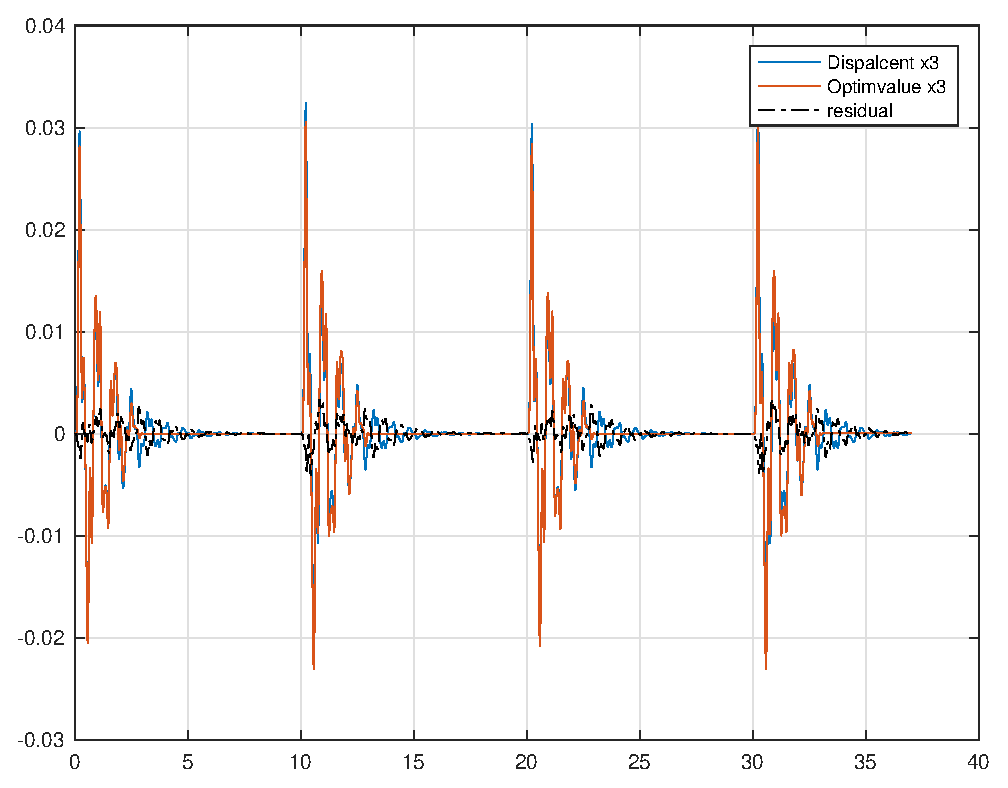
\includegraphics[width=0.45\textwidth]{residualfull3}}
	\caption{Comparison between the response of the model and the response of the 
	system free damping case}
	\label{fig:freedampingcase}
\end{figure}
\pagebreak
%
\subsection{Proportional damping case}
\label{subsec:proportionaldamping}
In this case, the procedure used to solve the problem raised in the case of 
free damping to obtain the parameters is used; changing some conditions.
We define damping through the equation (\ref{eq:proportionaldamping}) where it 
is possible to observe that this depends on the linear combination of the mass 
matrix multiply by constant and the stiffness matrix multiply by the another 
constant.
Then the search limits and first guess will be changed to search the mass 
values and the unknown constants.
The interesting property of this representation is the ability to perform modal 
decomposition on the system.
\begin{equation}
\label{eq:proportionaldamping}
	[C] = \alpha \cdot [M] + \beta \cdot [K]
\end{equation}
The optimization results are available in the table \ref{tab:proportionaldamping}.
%
\begin{table}[htb]
	\centering
	\begin{tabular}{SSSSSS}
	\toprule
	\multicolumn{1}{c}%
			{$m_1$} & {$m_2$} & {$m_3$} & {$g_v$} &	 {$\alpha$} & {$\beta$} \\
	\multicolumn{3}{c}{[\si{\kilo\gram}]}	& %
	\multicolumn{1}{c}{[\si{\volt}]} & %
	\multicolumn{2}{c}{[\si{\newton\second\per\meter}]} \\
	\midrule
       			1.5761   &  1.4970  & 1.1996  &  1.2094 &  1.6209   &  0.0001	\\
    \bottomrule
	\end{tabular}
	\caption{Optimizations results in proportional damping case}
	\label{tab:proportionaldamping}
\end{table}
%
%
%
\begin{figure}[htb]
\centering
	\subfloat[][\emph{residual.}]
		{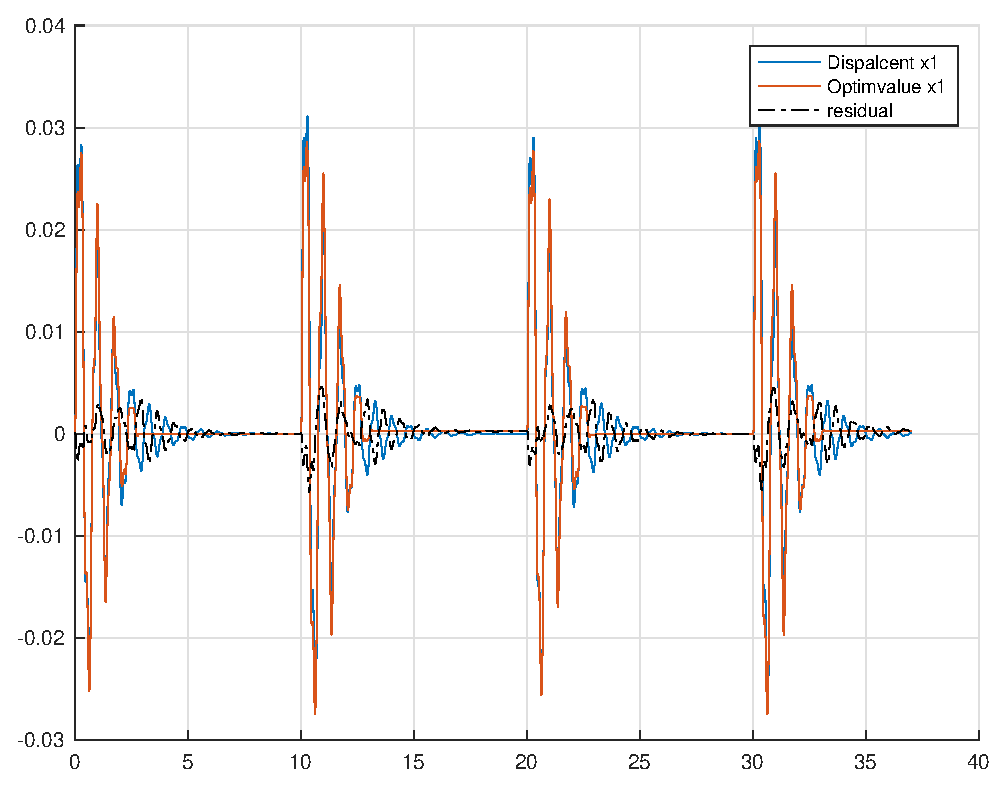
\includegraphics[width=0.45\textwidth]{residualpropdamp1}}	\,
	\subfloat[][\emph{residual.}]
		{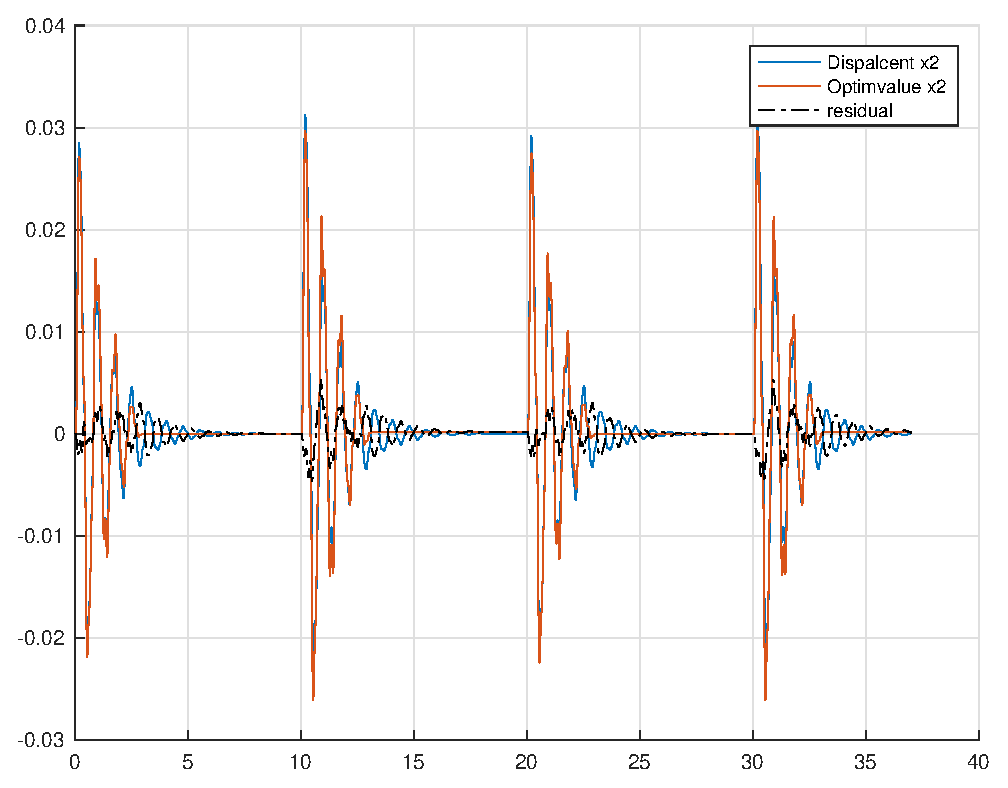
\includegraphics[width=0.45\textwidth]{residualpropdamp2}}	\\
	\subfloat[][\emph{residual.}]
		{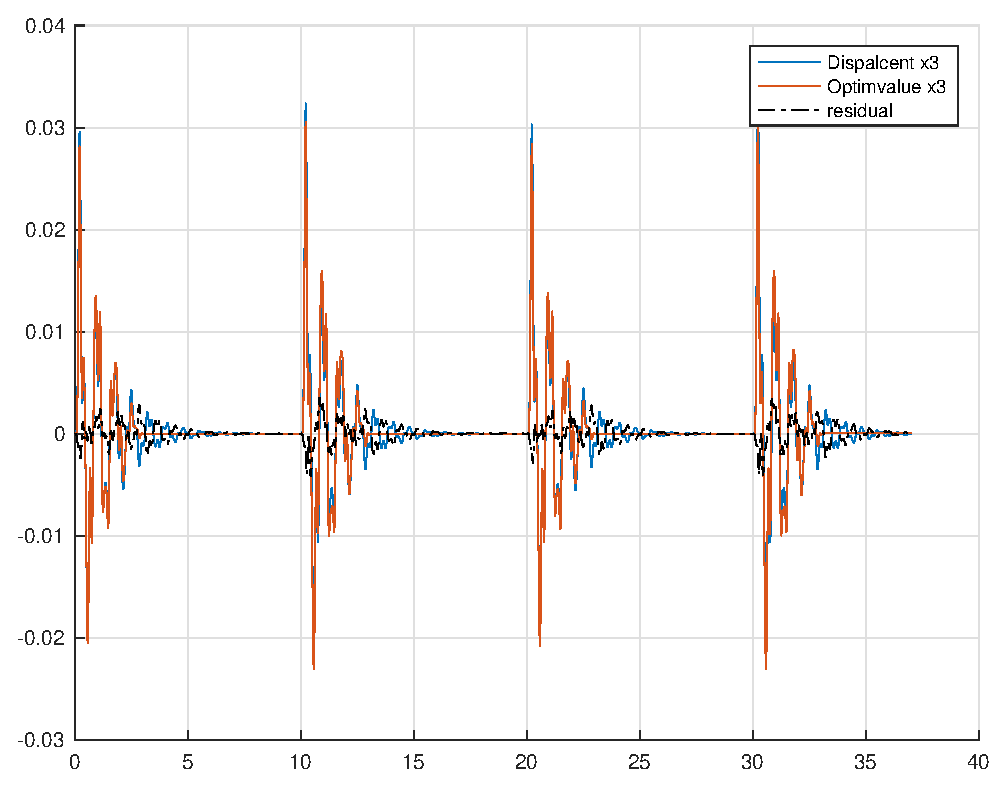
\includegraphics[width=0.45\textwidth]{residualpropdamp3}}	
	\caption{Comparison between the response of the model and the response of the system proportional damping case}
	\label{fig:proportionaldamping}
\end{figure}

%TODO describe the matrix C 
%The matrix [C] is:
\begin{equation}
\label{}
	[C] =
	\begin{bmatrix*}[r]
		 2.64026		&	-0.08550		 & 	 0.00000 	\\
		-0.08550 	&	 2.59748		 &	-0.08550		\\
		 0.00000 	&	-0.08550		 &	 2.07270		\\
	\end{bmatrix*}
\end{equation}
\pagebreak
%
\subsection{Comparison}
\label{subsec:comparison}
After fitting data with a model, you should evaluate the goodness of fit. 
The goodness of fit is calculated using the normalized root mean square error 
as the cost function.
In table \ref{tab:goodoffit} are aviable the percentages the measured output.
This method to assess goodness of fit for both linear and non linear parametric 
fits.
As is common in statistical literature, the term goodness of fit is used here 
in sense: ``good fit" might be a model where the data could reasonably have 
come from, given the assumptions of least-squares fitting.
\begin{table}[ht]
\centering
\begin{tabular}{lccc}
	\toprule
		 & $x_1$ [\%] & $x_2$ [\%] & $x_3$ [\%]\\
	\midrule
	% free damping result
	free damping case & 81.36 & 81.17 & 81.71 \\
	% proportianl damping result
	proportinal damping case & 81.36 & 81.17 & 81.56 \\
	\bottomrule
\end{tabular}
\caption{Result \emph{goodness of fit} measured output}
\label{tab:goodoffit}
\end{table}
%
\subsection{Multiple single DOF system case}
